% http://tex.stackexchange.com/questions/253007/marking-angles-in-a-parallelogram-congruent-using-tikz
\documentclass[tikz,border=7mm]{standalone}
\usetikzlibrary{angles}

\begin{document}
  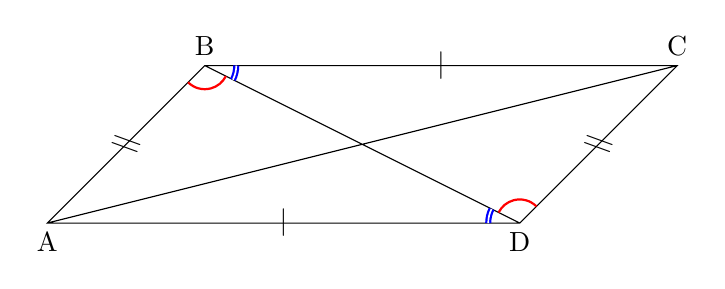
\begin{tikzpicture}[xslant=1,xscale=3,scale=2]
    \draw (0,0) rectangle
          (1,1) coordinate(C) node[above]{C} -- (0,0) coordinate(A) node[below]{A}
          (1,0) coordinate(D) node[below]{D} -- (0,1) coordinate(B) node[above]{B}
          (0.5,0) node {$|$} (0.5,1) node {$|$}
          (0,0.5) node[rotate=70] {$||$} (1,.5) node[rotate=70] {$||$}
          pic[draw,red,thick,angle radius=3mm] {angle = A--B--D}
          pic[draw,red,thick,angle radius=3mm] {angle = C--D--B}
          pic[draw,double,blue,thick,angle radius=4mm] {angle = B--D--A}
          pic[draw,double,blue,thick,angle radius=4mm] {angle = D--B--C};
  \end{tikzpicture}
\end{document}
